\documentclass[11pt]{article}
\usepackage[margin=1in]{geometry}
\usepackage{amsmath,amssymb}
\usepackage{booktabs}
\usepackage{graphicx}
\usepackage{pdfpages}
\usepackage{parskip}

\title{CAAM 37711 --- Homework 1 Solutions (Fall 2026)}
\author{Filippo Delzanno}

\newcommand{\results}[1]{../results/#1}

\begin{document}
\maketitle

\section*{Problems 1--3: Handwritten solutions}

\IfFileExists{theory/notes-HW1.pdf}{%
  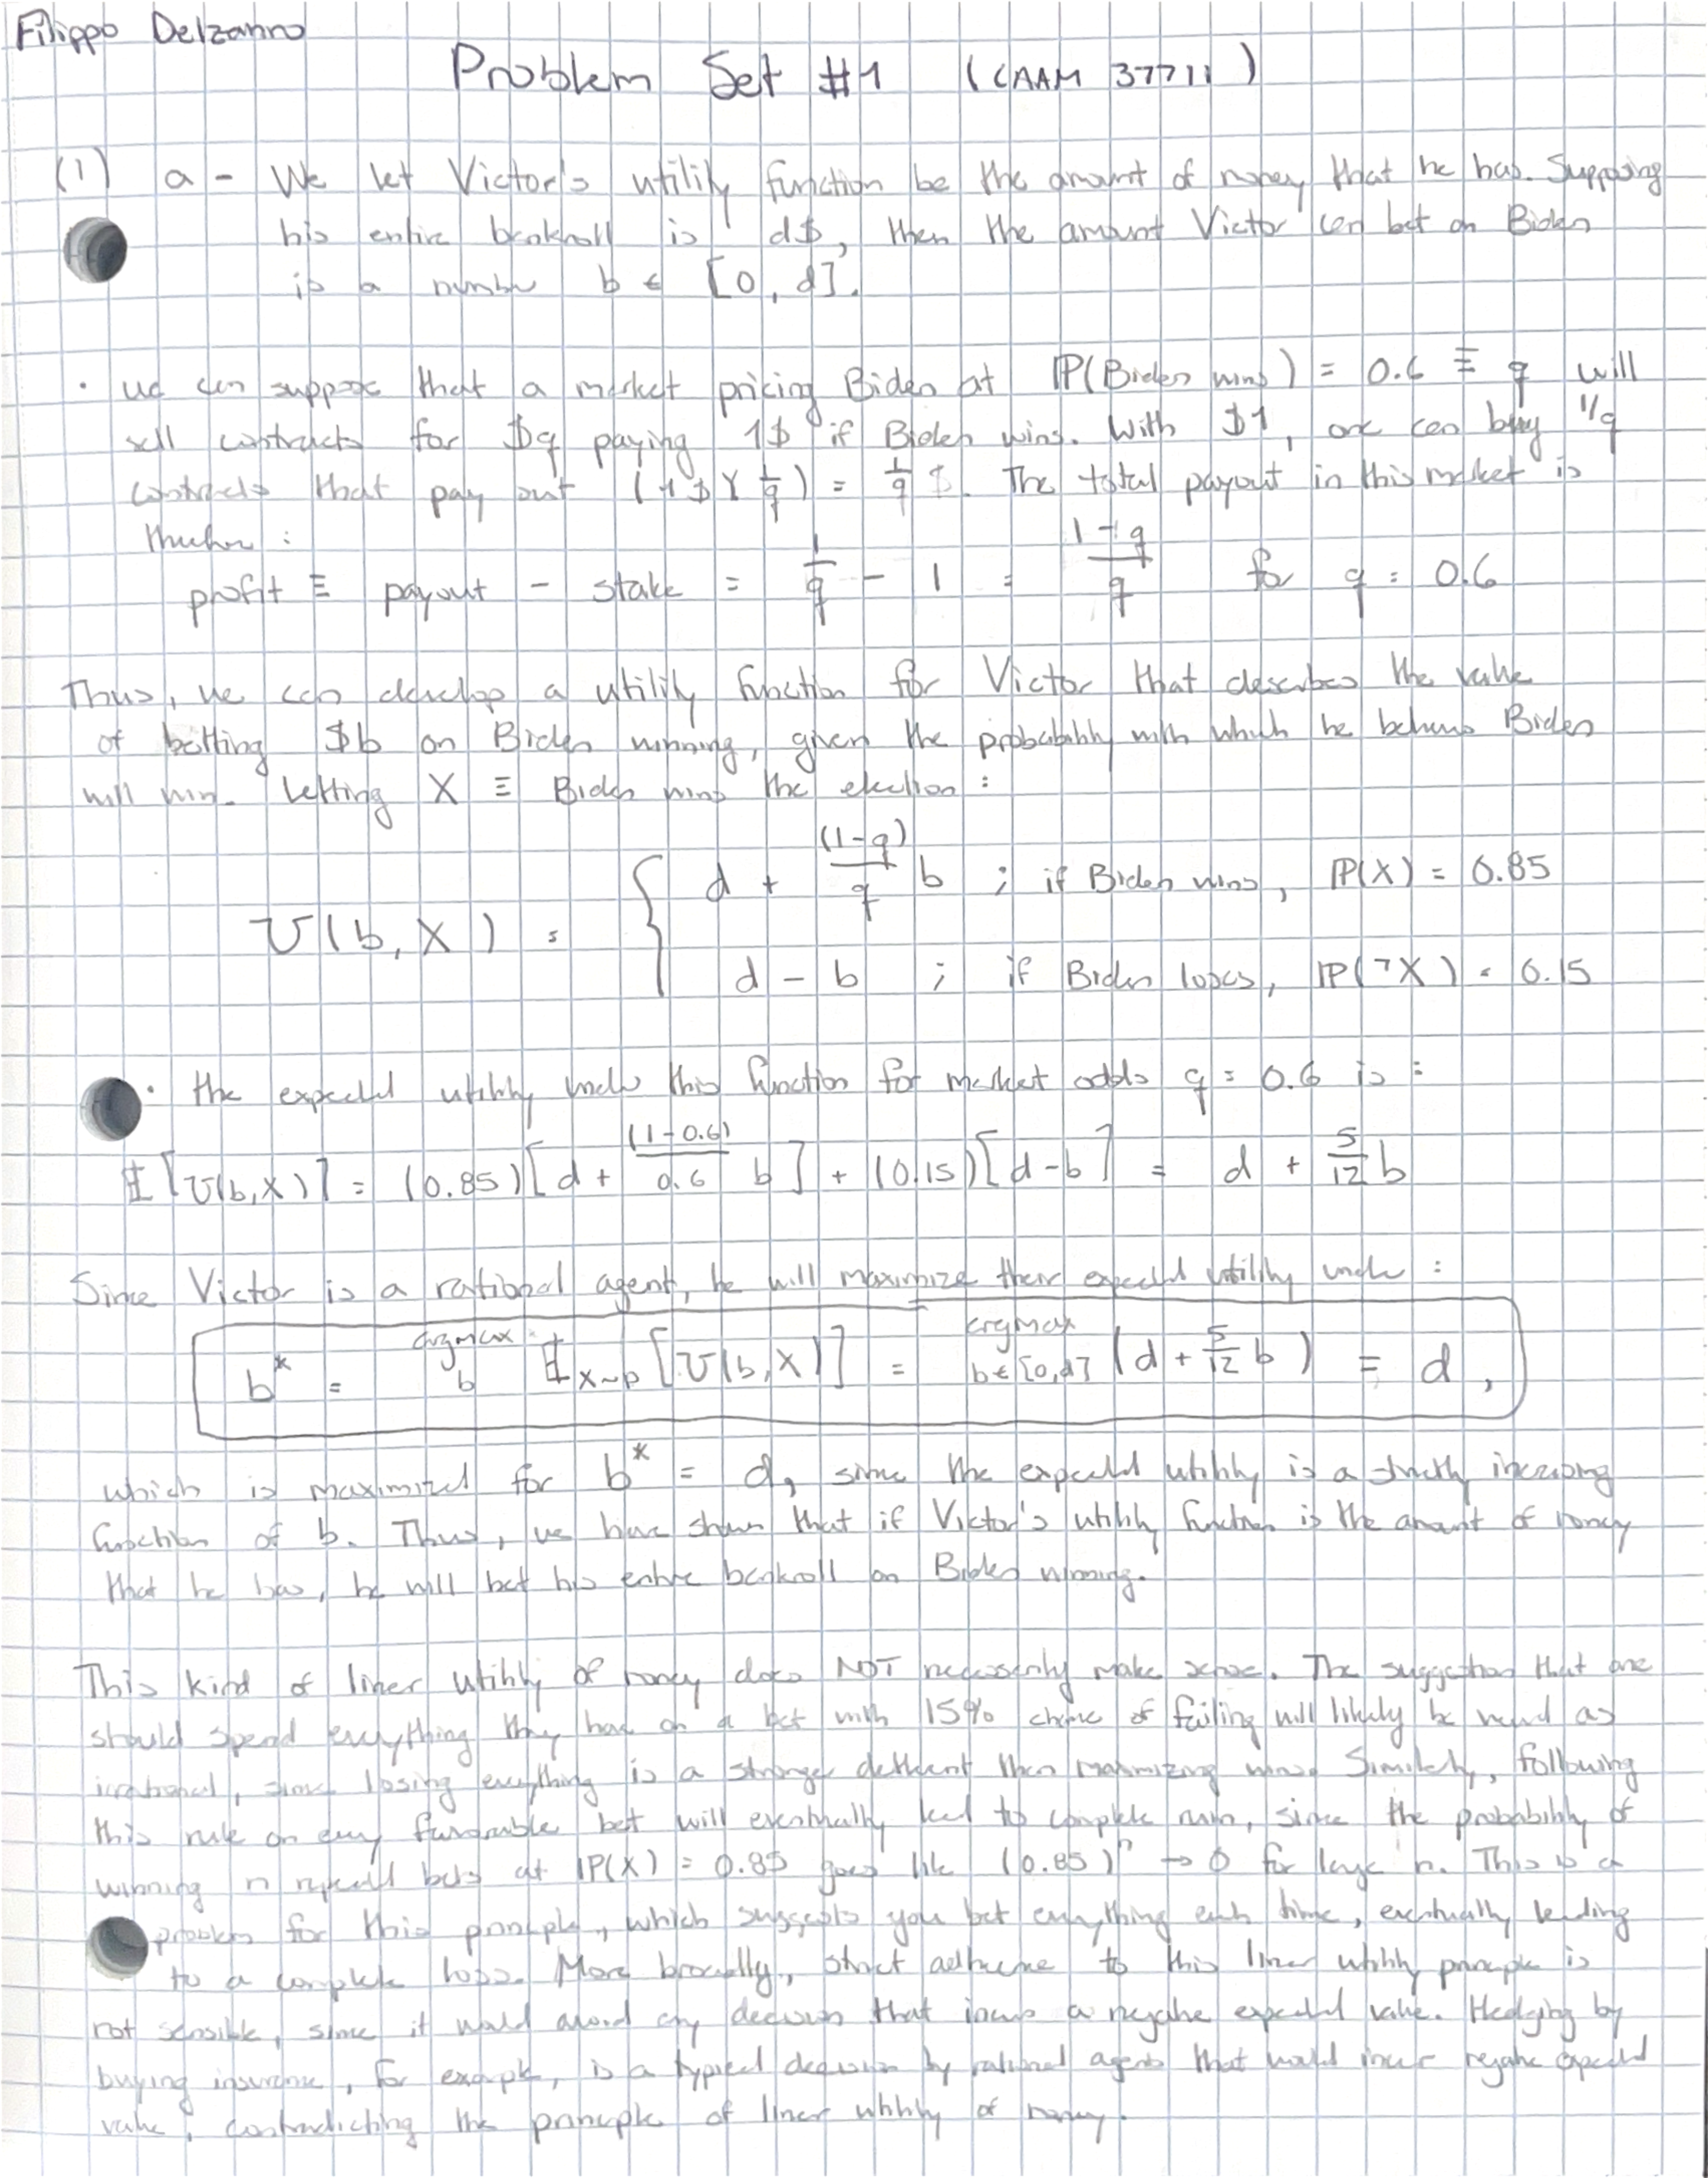
\includepdf[pages=-,pagecommand={\thispagestyle{empty}}]{theory/notes-HW1.pdf}%
}{%
  \bigskip\noindent\textbf{[Handwritten solutions for Problems 1--3 not yet added: place the scan at
  \texttt{homework-1/report/theory/notes-HW1.pdf} and rebuild.]}%
}

All code for this assignment is in the GitHub repository \texttt{https://github.com/fdelzanno/CAAM-37711}, under the \texttt{homework-1/} directory. See \texttt{README.md} for setup and run instructions.

\section*{Problem 4}

The problem recommends that we fit different regression models from the \texttt{sklearn} package. Following that recommendation, we will use the following models:
\begin{itemize}
    \item \textbf{Linear Regression}: fits a traditional linear model with corresponding weights by minimizing the squared error.
 
    \item \textbf{Support Vector Regression (SVR)}: SVR fits a function such that as many training points as possible lie within a ``tube'' in feature space of width $\pm\epsilon$ around it. The fit ignores errors inside the tube and penalizes errors outside in proportion to their size. We pass a regularization parameter $C$ that sets the tradeoff between fitting data closely and keeping the resulting function smooth (i.e., a larger $C$ penalizes points outside the tube more heavily). To capture nonlinear relationships, we use a radial basis function (RBF) kernel $K(x, x') = \exp\!\left(-\gamma \lVert x - x' \rVert^2\right)$. This measures the similarity between two points as a decreasing function of their distance such that the resulting prediction is a weighted sum of smooth, Gaussian ``bumps'' centered on a subset of the training points (called the support vectors). In this way, each prediction is mainly influenced by nearby training data. Since the kernel depends on distances in feature space, we standardize all four features to zero mean and unit variance before fitting to avoid a single feature dominating.
 
    \item \textbf{Decision Tree}: this regressor predicts the target by splitting the data into smaller groups sorted by particular characteristics of the features. At each step, the algorithm chooses the feature and threshold that best separate the data (i.e., the split that most reduces the squared error between the observations and the mean of their group). Since this splitting continues until a stopping rule is reached, the final groups (called leaves) will each predict the average \textbf{ale} of the training points it contains. This makes the fitted model a step function with abrupt jumps at the splitting thresholds. Since an unrestricted tree could continue to split until every leaf holds a single training point, we artificially limit the tree to stop at a depth of 4 (giving at most 16 leaves).
 
    \item \textbf{Neural Network}: predicts the target by passing the inputs through a series of layers made of simple computational units. Each unit takes a weighted sum of inputs, adds a constant (the bias), and applies a nonlinear activation function. In this case, we apply the rectified linear unit (ReLU), which outputs the value unchanged if it is positive and zero otherwise. Stacking layers of these units lets the network build up complex, nonlinear relationships from the pieces, creating an output that is a weighted combination of the last hidden layer's values. For this example, we will use two hidden layers of 32 units each. The weights and biases will start at random values and are adjusted iteratively by gradient descent to minimize the squared error between predictions and observed values. We allow up to 5{,}000 training iterations since we are dealing with a small dataset.
\end{itemize}
 
Since the SVR and neural network models are sensitive to the scale of their input features, a feature with a large numeric range can dominate the fit. To prevent this, we apply scikit-learn's \texttt{StandardScaler} to transform each feature into having zero mean and unit variance. Then, we combine the scaler and the model into a single \texttt{Pipeline} so that the means/standard deviations are computed from the training set only, and the same transformation is applied to the test data at prediction time. This should prevent information from the test set from leaking into the training data. Since linear regression and decision tree are unaffected by feature scaling, we do not apply this procedure to them.
 
To assess whether the computed residuals are approximately normal, we will follow the problem's suggestion: combine a QQ plot with a \texttt{scipy} normal test. The quantile-quantile (QQ) plot sorts the residuals from smallest to largest and plots each one against the value we would expect at that position if the data came from a normal distribution. These give us a visual check on the normality of the residuals, since normal residuals will lie on a straight line on the QQ plot. The formal test is the D'Agostino--Pearson test (\texttt{scipy.stats.normaltest}), which measures the residuals' skewness and kurtosis, compares each to the value expected under normality, and combines the two into a single statistic. The null hypothesis is that the residuals are drawn from a normal distribution, so a $p$-value below 0.05 is taken as evidence \textbf{against} normality. A large $p$-value means that the test finds no significant departure from normality.

\begin{figure}[h]
  \centering
  \includegraphics[width=0.8\textwidth]{\results{figures/p4_qqplots.png}}
  \caption{QQ plots of test residuals (points) against the normal distribution (red line).}
  \label{fig:qqplot}
\end{figure}

\begin{table}[h]
  \centering
  \input{\results{p4_table.tex}}
  \caption{Test RMSE and normality test of the test-set residuals ($n=27$).}
\end{table}

We fit four regression models (linear regression, SVR with an RBF kernel, a decision tree, and a neural network) to predict ALE from four features: anchor ratio, transmission range, node density, and iterations. We tested whether each model's residuals on a test set are approximately normal, and found that all three nonlinear models outperformed linear regression. Further, the D'Agostino--Pearson test rejected normality only for the linear model and failed to reject normality at the 0.05 significance level for the other three. This indicates that the relationship between the features and ALE is likely nonlinear and cannot be fully captured by a simple family of linear models.
 
These results suggest that the non-normality of the linear model's residuals is likely a symptom of model misspecification (as opposed to non-Gaussian noise in the data). Since linear models cannot capture the nonlinear structure in ALE, their systematic errors must remain in the residuals and distort their distribution. Indeed, the QQ plot of the linear model's residuals is convex, with a short lower tail and a long upper tail, indicative of right skew driven by a small number of large positive residuals. More flexible models can capture this structure, leaving residuals consistent with approximately normal noise.
 
Overall, the results are consistent with the common justification for squared error loss cited in the problem statement: that the fitted residuals are approximately normally distributed. This result comes with the caveat, however, that the model must be flexible enough to capture the underlying relationship of the data, and should be interpreted in the context of this small dataset. With only 27 test residuals per model, the normality test has limited power, and failing to reject normality in this test is not the same as showing that the residuals are truly normal. We have shown that approximate normality is an appropriate justification, but would need to repeat this procedure on a larger test sample to establish normality in the residuals with more confidence.

\section*{Problem 5}

\subsection*{Classification (Breast Cancer Wisconsin)}

As requested by the problem, we perform an 80/20 train-test split on the data.  We collect a baseline result using scikit-learn's \texttt{LogisticRegression} on the training data and measure prediction accuracy on the test sample. Then, we optimize two models: (a) logistic regression $f(x)=\sigma(w^\top x+b)$ and (b) probit regression $f(x)=\Phi(w^\top x+b)$ by minimizing a binary cross-entropy loss function (truncated to $[10^{-7},1-10^{-7}]$ to avoid numerical instabilities). We noticed that the training loss drops quickly in the first few epochs and then keeps decreasing slowly. Therefore, we report results for 200 epochs, at which point the loss has largely flattened, and a learning rate of 0.1.

\begin{table}[h]
  \centering
  \input{\results{p5_class_table.tex}}
  \caption{Test accuracy on the Breast Cancer test set.}
\end{table}

The SGD logistic model slightly exceeds the baseline (by 1 test observation), while the SGD probit model is slightly below it (by 1 test observation). Since the gaps are single test observations out of 114, they are within the variability that could be produced by varying the learning rate, number of epochs, or using different train/test splits. Note that the baseline also applies scikit-learn's default $\ell_2$ regularization, which the SGD models do not use (they are unregularized). This may account for part of the difference. Overall, the two model functions give very similar classifiers, as expected, since $\sigma$ and $\Phi$ are both smooth S-shaped maps from the real line to $(0,1)$.

\subsection*{Regression (ALE)}

As requested by the problem, we perform an 80/20 train-test split on the data. We collect a baseline result by applying scikit-learn's \texttt{LinearRegression} on the training data and computing the mean absolute error (MAE) on the test sample. Then, we optimize a Linear Regression model on both (a) the mean squared error loss and (b) the Student-$t$ negative log-likelihood with $\nu=5$ degrees of freedom and compare the mean absolute error on the test data using parameters learned from each loss function with the baseline result. By testing combinations of parameters, we determined that using 200 training epochs and a learning rate of 0.05 was enough to converge the model training loss to a sufficient plateau. 

\begin{table}[h]
  \centering
  \input{\results{p5_reg_table.tex}}
  \caption{MAE on the ALE test set ($n=22$).}
\end{table}

Both SGD-trained models achieve a test MAE essentially identical to the baseline: the MSE-trained model is slightly worse, and the Student-$t$-trained model is slightly better. These gaps are less than $10^{-3}$ on only 22 test observations, so they are well within the variability that could be produced by changing the number of epochs and learning rate, or using a different train/test split. From this data alone, we cannot conclude that either loss is better. Since the MSE-trained SGD model minimizes the same loss function as \texttt{LinearRegression}, it should approach the least-squares solution. This is consistent with what we see for the MSE, and the small difference likely reflects the finite training we use for SGD or batch sampling noise. As noted in the problem statement, the Student-$t$ distribution has heavier tails, so minimizing its loss function will differ from squared error mainly for large residuals. When we looked at the residuals of the linear model in Problem 4 (Fig.~\ref{fig:qqplot}), we saw that they lie between about $-0.35$ and $0.9$, with most within $\pm 0.4$. Thus, we do not expect the heavy-tailed loss to change the fit much, which is consistent with our observation that its test MAE is nearly identical to that of the MSE-trained model.

\clearpage

\end{document}
